\documentclass{standalone}
\usepackage[utf8]{inputenc}
\usepackage{pgfplots}
\usepgfplotslibrary{groupplots}
\pgfplotsset{compat=1.18}


% function which draws little triangles inside the loglog plot
% example usage: \logLogSlopeTriangle{0.5}{0.2}{0.85}{1}{black}{0};
% 0.5 ...... x-coordinate of the corner
% 0.2 ...... scaling
% 0.85 .... y-coordinate of the corner
% 1 ......... length of the vertical line
% black ... color of the triangle
% 0 ........ (boolean) if we want to flip the triangle or not
\newcommand{\logLogSlopeTriangle}[6]{
    \pgfplotsextra
    {
        \pgfkeysgetvalue{/pgfplots/xmin}{\xmin}
        \pgfkeysgetvalue{/pgfplots/xmax}{\xmax}
        \pgfkeysgetvalue{/pgfplots/ymin}{\ymin}
        \pgfkeysgetvalue{/pgfplots/ymax}{\ymax}

        \pgfmathsetmacro{\xArel}{#1}
        \pgfmathsetmacro{\yArel}{#3}
        \pgfmathsetmacro{\xBrel}{#1-#2}
        \pgfmathsetmacro{\yBrel}{\yArel}

        \pgfmathsetmacro{\lnxB}{\xmin*(1-(#1-#2))+\xmax*(#1-#2)} % in [xmin,xmax].
        \pgfmathsetmacro{\lnxA}{\xmin*(1-#1)+\xmax*#1} % in [xmin,xmax].
        \pgfmathsetmacro{\lnyA}{\ymin*(1-#3)+\ymax*#3} % in [ymin,ymax].
        \pgfmathsetmacro{\lnyC}{\lnyA+#4*(\lnxA-\lnxB)}

        % Check if flip is true or false using \ifnum (0 = false, 1 = true)
        \ifnum#6=1
            % Flipped version
            \pgfmathsetmacro{\xCrel}{\xBrel}
            \pgfmathsetmacro{\yCrel}{(\lnyC-\ymin)/(\ymax-\ymin)}

            % Define coordinates for the flipped triangle
            \coordinate (A) at (rel axis cs:\xArel,\yArel);
            \coordinate (B) at (rel axis cs:\xBrel,\yBrel);
            \coordinate (C) at (rel axis cs:\xCrel,\yCrel);

            % Draw flipped slope triangle.
            \draw[#5] (A)-- node[pos=0.5,anchor=north] {1} (B)-- node[pos=0.5,anchor=east] {#4}
               (C)-- cycle;
        \else
            % Non-flipped version
            \pgfmathsetmacro{\xCrel}{\xArel}
            \pgfmathsetmacro{\yCrel}{\yArel - (#4 * (\lnxA-\lnxB)/(\ymax-\ymin))}

            % Define coordinates for the non-flipped triangle
            \coordinate (A) at (rel axis cs:\xArel,\yArel);
            \coordinate (B) at (rel axis cs:\xBrel,\yBrel);
            \coordinate (C) at (rel axis cs:\xCrel,\yCrel);

            % Draw non-flipped slope triangle.
            \draw[#5] (A)-- node[pos=0.5,anchor=south] {1} (B)--
               (C)-- node[pos=0.5,anchor=west] {#4} cycle;
        \fi
    }
}

\newcommand{\colorI}{magenta}
\newcommand{\colorII}{cyan}
\newcommand{\colorIII}{red}
\newcommand{\colorIV}{blue}

\begin{document}

\newcommand{\subfigwidth}{9.5cm}  % Define the width of the subfigures
\newcommand{\subfigheight}{8cm} % Define the height of the subfigures


\begin{tikzpicture}

% read data from tables and define precomputed slope and intercept for each dataset

% upper left figure
\pgfplotstableread{
x y1 y2
0.400 7.92e-08 2.92e-09
0.300 4.81e-08 1.71e-09
0.200 2.38e-08 8.08e-10
0.100 7.17e-09 2.24e-10
0.050 2.16e-09 6.20e-11
0.020 4.41e-10 1.14e-11
}\upperleft
\newcommand{\slopeupperleftI}{1.73}
\newcommand{\interceptupperleftI}{3.88e-07}
\newcommand{\slopeupperleftII}{1.85}
\newcommand{\interceptupperleftII}{1.59e-08}

% upper right figure
\pgfplotstableread{
x y1 y2
0.400 8.69e-08 6.42e-09
0.300 5.07e-08 3.73e-09
0.200 2.37e-08 1.74e-09
0.100 6.48e-09 4.69e-10
0.050 1.77e-09 1.27e-10
0.020 3.18e-10 2.25e-11
}\upperright
\newcommand{\slopeupperrightI}{1.87}
\newcommand{\interceptupperrightI}{4.83e-07}
\newcommand{\slopeupperrightII}{1.89}
\newcommand{\interceptupperrightII}{3.62e-08}

% lower left figure
\pgfplotstableread{
x y1 y2
0.400 1.54e-07 8.80e-08
0.300 1.15e-07 6.14e-08
0.200 7.62e-08 3.70e-08
0.100 3.77e-08 1.55e-08
0.050 1.87e-08 6.53e-09
0.020 7.39e-09 2.08e-09
}\lowerleft
\newcommand{\slopelowerleftI}{1.01}
\newcommand{\interceptlowerleftI}{3.89e-07}
\newcommand{\slopelowerleftII}{1.25}
\newcommand{\interceptlowerleftII}{2.77e-07}

% lower right figure
\pgfplotstableread{
x y1 y2
0.400 1.63e-07 1.05e-07
0.300 1.12e-07 6.97e-08
0.200 6.55e-08 3.89e-08
0.100 2.63e-08 1.44e-08
0.050 1.06e-08 5.31e-09
0.020 3.16e-09 1.42e-09
}\lowerright
\newcommand{\slopelowerrightI}{1.32}
\newcommand{\interceptlowerrightI}{5.45e-07}
\newcommand{\slopelowerrightII}{1.44}
\newcommand{\interceptlowerrightII}{3.93e-07}

% =====================
% the figure starts here

\begin{groupplot}[
        group style={
        {group size=2 by 2}}, height=6cm, width=.5\textwidth,legend style={
        transpose legend,
        legend columns=2,
        % draw=none, % if you want to hide the frame around legend
        /tikz/every even column/.append style={column sep=5pt}},
        xlabel={x-axis label},
        xmode=log,
        ymode=log,
        x dir=reverse,
        % y label style={at={(0.1,1.075)}},
        % ylabel style={rotate=-90},
        width=\subfigwidth, height=\subfigheight,
        xmin=0.01, xmax=0.5,
        enlarge x limits=0.05,
        ymin=1e-9, ymax=3e-7,
        enlarge y limits=0.1,
        grid=both,
        grid style={color=gray!30},
        legend pos=south west,
        legend style={font=\footnotesize},
        tickpos=left,
        ytick align=inside,
        xtick align=inside,
        x tick label style={ align=center},
        xticklabel shift=1pt,
        ]

% =====================
% first row

    \nextgroupplot[%title={Title}, 
        legend to name=groupLegendPatients,
        ylabel={y-axis label},
        ymin=1e-11, ymax=1e-7,
        ]
        \addplot [only marks, mark=*, color=\colorI, thick, mark options={fill=\colorI}] table [x=x, y=y1] {\upperleft} ;
        \addplot[domain=0.01:0.5, color=\colorI, dashed]
        {\interceptupperleftI * x^(\slopeupperleftI)};
        
        \addplot [only marks, mark=*, color=\colorII, thick, mark options={fill=\colorII}] table [x=x, y=y2] {\upperleft} ;
        \addplot[domain=0.01:0.5, color=\colorII, dashed]
        {\interceptupperleftII * x^(\slopeupperleftII)};

        \logLogSlopeTriangle{0.8}{0.2}{0.8}{2}{black}{0};
            
     \nextgroupplot[
        ymin=1e-11, ymax=1e-7,
     ]
        \addplot [only marks, mark=*, color=\colorI, thick, mark options={fill=\colorI}] table [x=x, y=y1] {\upperright} ;
        \addplot[domain=0.01:0.5, color=\colorI, dashed]
        {\interceptupperrightI * x^(\slopeupperrightI)};
        
        \addplot [only marks, mark=*, color=\colorII, thick, mark options={fill=\colorII}] table [x=x, y=y2] {\upperright} ;
        \addplot[domain=0.01:0.5, color=\colorII, dashed]
        {\interceptupperrightII * x^(\slopeupperrightII)};
        
        \logLogSlopeTriangle{0.8}{0.2}{0.8}{2}{black}{0};
        

% =====================
% second row

    \nextgroupplot[
    yshift=-3\pgfkeysvalueof{/pgfplots/every axis title shift},
        ylabel={y-axis label},
        ]
        \addplot [only marks, mark=*, color=\colorIII, thick, mark options={fill=\colorIII}] table [x=x, y=y1] {\lowerleft} ;
        \addplot [only marks, mark=triangle*, color=\colorIV, thick, mark options={fill=\colorIV}] table [x=x, y=y2] {\lowerleft} ;
        
        \addplot[domain=0.01:0.5, color=\colorIII, dashed]
            {\interceptlowerleftI * x^(\slopelowerleftI)};
        \addplot[domain=0.01:0.5, color=\colorIV, dashed]
            {\interceptlowerleftII * x^(\slopelowerleftII)};
            
         \logLogSlopeTriangle{0.5}{0.2}{0.85}{1}{black}{0};
         \logLogSlopeTriangle{0.4}{0.2}{0.3}{1.5}{black}{1};
            
            
      \nextgroupplot[
      yshift=-3\pgfkeysvalueof{/pgfplots/every axis title shift},
      ]
        \addplot [only marks, mark=*, color=\colorIII, thick, mark options={fill=\colorIII}] table [x=x, y=y1] {\lowerright} ;
        \addplot [only marks, mark=triangle*, color=\colorIV, thick, mark options={fill=\colorIV}] table [x=x, y=y2] {\lowerright} ;
        
        \addplot[domain=0.01:0.5, color=\colorIII, dashed]
            {\interceptlowerrightI * x^(\slopelowerrightI)};
        \addplot[domain=0.01:0.5, color=\colorIV, dashed]
            {\interceptlowerrightII * x^(\slopelowerrightII)};
        \logLogSlopeTriangle{0.5}{0.2}{0.85}{1}{black}{0};
        \logLogSlopeTriangle{0.4}{0.2}{0.3}{1.5}{black}{1};

\end{groupplot}

% legend above
\node at ($(group c1r1.north)!0.5!(group c2r1.north)$) [above, yshift=\pgfkeysvalueof{/pgfplots/every axis title shift}] {
    \begin{tikzpicture}
        \begin{axis}[
            hide axis, % Hide the axis
            xmin=0, xmax=1, ymin=0, ymax=1,
            legend columns=2,
            legend style={
                draw=black, % Adds a black frame around the legend
                fill=white, % Background color (optional)
                /tikz/every even column/.append style={column sep=0.5cm},
                % font=\footnotesize, % Adjust font size if needed
                column sep=1ex, % Space between columns
                nodes={anchor=west}, % Align text to the left
            },
        ]
            \addlegendimage{thick, \colorI, mark=*, mark options={fill=\colorI, solid}, legend image post style={dashed}}
            \addlegendentry{convergence 1}
            \addlegendimage{thick, \colorII, mark=*, mark options={fill=\colorII, solid}, legend image post style={dashed}}
            \addlegendentry{convergence 2}

        \end{axis}
    \end{tikzpicture}
};

% legend below
\node at ($(group c1r2.south)!0.5!(group c2r2.south)$) [below, yshift=-5\pgfkeysvalueof{/pgfplots/every axis title shift}] {
    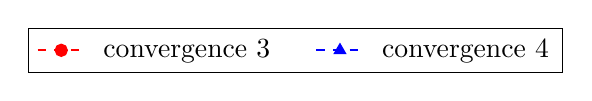
\begin{tikzpicture}
        \begin{axis}[
            hide axis, % Hide the axis
            xmin=0, xmax=1, ymin=0, ymax=1,
            legend columns=2,
            legend style={
                draw=black, % Adds a black frame around the legend
                fill=white, % Background color (optional)
                /tikz/every even column/.append style={column sep=0.5cm},
                % font=\footnotesize, % Adjust font size if needed
                column sep=1ex, % Space between columns
                nodes={anchor=west}, % Align text to the left
            },
        ]
            \addlegendimage{thick, \colorIII, mark=*, mark options={fill=\colorIII, solid}, legend image post style={dashed}}
            \addlegendentry{convergence 3}
            \addlegendimage{thick, \colorIV, mark=triangle*, mark options={fill=\colorIV, solid}, legend image post style={dashed}}
            \addlegendentry{convergence 4}

        \end{axis}
    \end{tikzpicture}
};

\node at ([below,yshift=-4\pgfkeysvalueof{/pgfplots/every axis title shift}]group c1r1.south) {
    (a) Caption A
};
\node at ([below,yshift=-4\pgfkeysvalueof{/pgfplots/every axis title shift}]group c2r1.south) {
    (b) Caption B
};
\node at ([below,yshift=-4\pgfkeysvalueof{/pgfplots/every axis title shift}]group c1r2.south) {
    (c) Caption C
};
\node at ([below,yshift=-4\pgfkeysvalueof{/pgfplots/every axis title shift}]group c2r2.south) {
    (d) Caption D
};

\end{tikzpicture}

\end{document}
